\section{Deep and shallow semantic construction}
\label{sec:motivation}

We start with an informal discussion of some toy \rmrs s, which are
meant to illustrate how \rmrs\ can be used to represent partial
semantic information, and why people find it useful for this purpose.

\newcommand{\sem}[1]{\mathsf{#1}}
\newcommand{\sempred}[1]{\mathrm{#1}}

Consider the following sentence:
\begin{examples}
  \item Every fat cat chased some dog.
\end{examples}

This sentence exhibits several kinds of ambiguity, including a scope
ambiguity between ``every fat cat'' and ``some dog'' and lexical
ambiguities of the words ``cat'' and ``dog'' (which have 8 and 7 noun
senses according to Wordnet, respectively).  Two of these readings are
shown as logical forms below; they can be represented as trees as
shown in Fig.~\ref{fig:1}.

\begin{examples}
\item $\sem{\_every\_q\_1}(x, \sem{\_fat\_j\_1}(e',x) \wedge
    \sem{\_cat\_n\_1}(x), \sem{\_some\_q\_1}(y, \sem{\_dog\_n\_1}(y),
    \sem{\_chased\_v\_1}(e,x,y)))$
\label{ex:fat-cat-1}
\item $\sem{\_some\_q\_1}(y, \sem{\_dog\_n\_2}(y),
\sem{\_every\_q\_1}(x, \sem{\_fat\_j\_1}(e',x) \wedge
    \sem{\_cat\_n\_2}(x), 
    \sem{\_chased\_v\_1}(e,x,y)))$
\label{ex:fat-cat-2}
\end{examples}


\begin{figure*}[t]
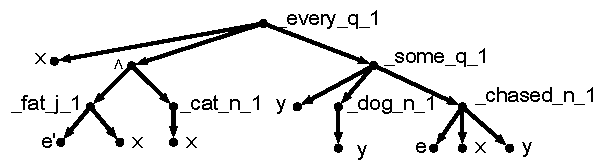
\includegraphics[width=6cm]{pic-cat-chased-dog}
\hspace{1cm}
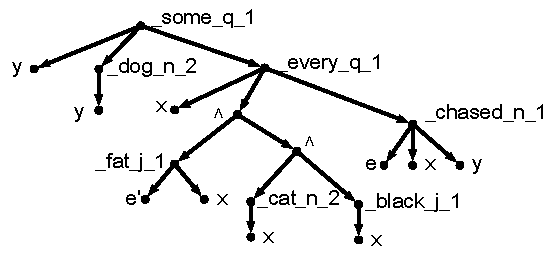
\includegraphics[width=6cm]{pic-cat-chased-dog-2}
\caption{Structure trees of the semantic representations (\ref{ex:fat-cat-1}) and
  (\ref{ex:fat-cat-2}). \label{fig:1}}
\end{figure*}


Now imagine that we are trying to extract semantic information from
the output of a part-of-speech tagger by using the word lemmas as
lexical predicate symbols.  Such a semantic representation is highly
partial, as it will not say anything about predicate-argument
relations, or resolve lexical ambiguity -- it will use predicate
symbols such as $\sempred{\_cat\_n}$, which might resolve to the
predicate symbols $\sem{\_cat\_n\_1}$ or $\sem{\_cat\_n\_2}$ in the
complete semantic representation.  (Notice that we are using different
fonts for the ambiguous and unambiguous predicate symbols.)  We can
express this information in \rmrs\ as follows.

\begin{examples}
\item \label{ex:cat-pos}
$l_1:a_1:\sempred{\_every\_q}(x)$, \\
$l_{41}:a_{41}:\sempred{\_fat\_a}(e')$,\\
$l_{42}:a_{42}:\sempred{\_cat\_n}(x_3)$\\
$l_5:a_5:\sempred{\_chased\_v}(e_{past})$, \\
$l_6:a_6:\sempred{\_some\_q}(x_4)$, \\
$l_9:a_9:\sempred{\_dog\_n}(x_5)$
\end{examples}

This \rmrs\ consists of six \emph{elementary predications} (EPs), one
for each word lemma in the sentence; each of them is prefixed by a
\emph{label} and an \emph{anchor}, which are essentially variables
that refer to nodes in the trees in Fig.~\ref{fig:1}.  We can say that
the two trees \emph{satisfy} this \rmrs\ because it is possible to map
the labels and anchors into each tree in such a way that the label of
the node they are mapped to is consistent with the label specified in
the elementary predication.  For instance, the first tree satisfies
the \rmrs\ because we can map $l_1$ and $a_1$ to the root of that
tree, and the root label $\sem{\_every\_q\_1}$ is consistent with the
EP predicat $\sempred{\_every\_q}$.

There are of course many other trees (and thus, fully specific
semantic representations such as (\ref{ex:fat-cat-1})) that are
described equally well by the same \rmrs; this is not surprising,
given that the semantic information we got from the POS tagger is so
incomplete.  If we have more information, say information about the
predicate-argument structure and semantic dependencies from a partial
parser such as \todo{what? CASS?}, we can represent these in a more
detailed \rmrs, as follows:

\begin{examples}
\item 
$l_1:a_1:\sempred{\_every\_q}(x)$, \\
$l_{41}:a_{41}:\sempred{\_fat\_a}(e')$,\\
$l_{42}:a_{42}:\sempred{\_cat\_n}(x_3)$\\
$l_5:a_5:\sempred{\_chased\_v}(e_{past})$, \\
$l_6:a_6:\sempred{\_some\_q}(x_4)$, \\
$l_9:a_9:\sempred{\_dog\_n}(x_5)$
\todo{add more stuff with ARG and equalities here}
\label{ex:cat-partial-parser}
\end{examples}

This \rmrs\ uses two new types of atoms.  Atoms of the form $x=y$
express that the two variables $x$ and $y$ should really be the same;
in the example, the \rmrs\ uses two variable names $x$ and $x'$, which
are mapped to the same variable $x$ in Fig.~\ref{fig:1}.  \todo{I'm
  making these names up -- adjust to RMRS.}  Atoms of the form
$\ARG_i(a,x)$ and $\ARG_i(a,h)$ express that a node representing the
variable $x$ or a node denoted by the \emph{hole} $h$ is the $i$-th
child of the node to which the anchor $a$ refers.  The separation of
EPs and $\ARG$ atoms is perhaps the most important difference between
\rmrs\ and earlier underspecification formalisms such as \mrs\ and
dominance graphs, which required that a predicate and its arguments
had to be specified together.  \rmrs\ goes beyond these formalisms in
expressive power, especially if we allow atoms of the form
$\ARG_{\{2,3\}}(a,x)$ to express uncertainty as to whether $x$ is the
second or third child of the anchor $a$.

Notice also that the labels of the EPs for ``fat'' and ``cat'' are
stipulated to be equal in the \rmrs, whereas the anchors are not.
In the tree, it is the anchors that are mapped to the nodes with the
labels $\sem{\_fat\_a\_1}$ and $\sem{\_cat\_n\_1}$; the label is
mapped to the conjunction node just above them.  In other words, the
role of the anchor in an EP is to carry the predicate and connect to
the arguments; the role of the label is to connect the EP to the
surrounding formula.  The use of equal labels for two EPs stems from
\mrs, where intersective modification was also modeled by using two
EPs with the same label.

Finally, here is an \rmrs\ that could be derived from a deep grammar
such as the ERG:

\begin{examples}
\item $l_1:a_1\handel\mbox{\_every\_q\_1}(x_1),$\\
\hspace*{0.1in}$\mbox{RSTR}(a_1,h_2),
\mbox{BODY}(a_1,h_3)$\\ 
$l_{41}:a_{41}\handel\mbox{\_fat\_j\_1}(e'), \mbox{ARG1}(a_{41},x_2)$\\
$l_{42}:a_{42}\handel\mbox{\_cat\_n\_1}(x_3)$\\
$l_5:a_5\handel\mbox{\_chase\_v\_1}(e_{spast})$,\\
\hspace*{0.1in}$\mbox{ARG1}(a_5,x_4),
\mbox{ARG2}(a_5,x_5)$\\ 
$l_6:a_6\handel\mbox{\_some\_q\_1}(x_6)$,\\
\hspace*{0.1in}$\mbox{RSTR}(a_6,h_7),
\mbox{BODY}(a_6,h_8)$\\ 
$l_9:a_9\handel\mbox{\_dog\_n\_1}(x_7)$\\
$h_2=_q l_{42}, l_{41}=l_{42}, h_7 =_q l_9$\\
$x_1=x_2, x_2=x_3, x_3=x_4,$\\
$x_5=x_6, x_5=x_7$
\todo{fix RSTR and BODY to ARG1 and ARG2? or talk about it in the text?}
\label{ex:cat-erg}
\end{examples}

This is now an extremely detailed underspecified representation of the
different semantic representations of the sentence, which is
essentially a notational variant of the \mrs\ that the ERG would
derive.  Notice the use of atoms like $h_2 \qeq l_{42}$, which specify
a kind of ``outscopes'' relationship between the hole and the label,
and can be used to underspecify the scope of the two quantifiers.

In summary, \rmrs\ is a formalism for representing partial information
about semantic representations.  It generalizes \mrs\ in that it can
represent the output of a deep grammar in a way that is a notational
variant of \mrs; but in cases in which a deep grammar is not
available, it can be used to capture whatever partial semantic
information a shallower NLP tool was able to provide.  \rmrs\ is
designed to serve as a generic formalism for partial semantic
representations which abstracts over the details of different NLP
tools and allows us to represent, process, and compare information
from different tools in the same formalism.  In the long run, it could
also be a platform for incrementally enriching partial information
such as (\ref{ex:cat-pos}) in order to eventually approximate more
detailed representations such as (\ref{ex:cat-partial-parser}).

\todo{Leidensdruck!}

%%% Local Variables: 
%%% mode: latex
%%% TeX-master: "rmrs-08"
%%% End: 
